\chapter{Array Evaluation}
\label{chap:aev}
\section{Overview}
As stated in chapter \dots the geometry of a microphone array
has a impact on the performance of beamforming.
The goal is to find a well suited array geometry for the detection and tracking of
Drones.
To achieve this, first some array geometries have been simulated and then
a prototype was built to gather information on how they perform in reality.
Then the real data were compared to the simulated data to
confirm the validity of the simulation.
In the next step the findings of the prototypes and simulations
were used to come up with a final array design.

By analyzing the sound of some commercially available drones
a desired frequency range of 500 to 2000 hz was set.
This range includes most of the sound's energy.

The array geometry has some constraints,
such as the number of microphones and the mechanical feasibility.
As stated in \ref*{chap:AqqSys} the maximum number of microphones
in an array is 32.

To compare different array geometries, several simulations
were ran for each array.
The simulated data was then ran through the beamforming
algorithm.
The steering angles are based on a grid with $-180^\circ \leq \phi < 180\circ$ and
$0^\circ \leq \theta \leq 180^\circ$ with a spacing of $1^\circ$.
For each point in this grid the power over the desired frequency band is calculated.
Displaying the result leads to an image like Figure \ref*{aev:fig:gridEx}.
The visualizations may be misleading depending on the angle.
This is a result from the projection of the semisphere onto a 2-d surface.
\begin{figure}
	\centering
	%    \includegraphics[width=0.25\textwidth]{mesh}
	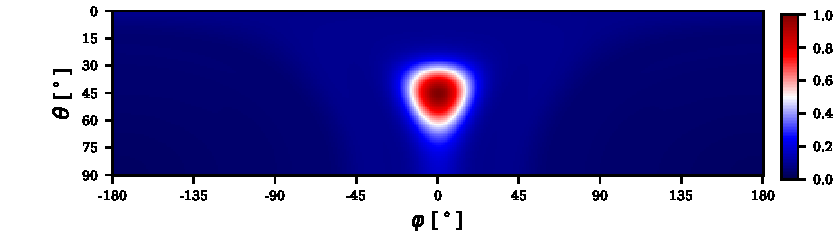
\includegraphics[]{images/5_array_evaluation/0.3_0.79.pdf}
	\caption{$G(\phi, \theta)$ for $-180 \leq \phi \leq 180$ and $0 \leq \theta \leq 90$.
	Red blob represents the mainlobe where the power is bigger than the half of the 
	maximum power.}
	\label{aev:fig:gridEx}
\end{figure}
\section{Metrics}
TO evaluate the performance of an array several metrics are used.
In \todo{Cite Array design s40430-018-1275-5-1, array design comparisons} the
main beam-width is proposed.
\todo{cite Circ array drone trackings13638-019-1632-9} is using the ratio
between the main lobe power and the side lobe power.
Another measure related to the main lobe with is the main lobe area.s
The main lobe is defined as all the points around the peak where their value
is greater than half the peaks value. \todo{besser englisch}

\subsection{Area}
Since the grid resulting from the beamforming represents spherical function
simply taking the sum of all the gridpoints from the mainlobe
would deliver false results.
So each grid point is normalized by the surface element of a sphere
\begin{equation}
	dA = r \sin\theta \, d\phi \cdot r d\theta.
\end{equation}
The area of the mainlobe determines how good different sources can be separated.
With a big mainlobe area two close sources may lead to one bigger mainlobe instead
of two separable ones.
Since the area is calculated with for $\theta < 90^\circ$, the areas calculated
for peaks close to that border are not the actual areas when looking at the 
full angular range.

\subsection{Peak Average Power ratio}
The Peak Average Power ratio is the ratio between the peak power and
the average power over the whole grid.
The results from the projection are compensated by weighting
the power at each grid cell with the area of that grid cell.
With these considerations the PAP ratio is defined as
\begin{equation}
	PAP = \frac{\max \, P(\phi, \theta)}{\sum_{\phi, \theta}^{} P(\phi, \theta) dA(\phi, \theta)}.
\end{equation}
A high PAP ratio is desired, since it means that little power is leaking 
into other directions than the real \acrshort{doa}.
\section{Array Geometry}
In \todo{cite} the authors use a circular array to detect and track drones.
They however did not gave any reasoning no why the chose a circular array.
\cite{bandkProducts}
In \cite{arr1} different array types are compared and measured.
The best scores are reached with the Underbrink style array, a combination
of multiple circular arrays.
They also included several spiral based arrays
Based on this three main groups of arrays were further analyzed,
the circular array, an adaption of the underbrink array, and a archimedes
spiral array.
\subsection{Circular Array}
The circular array is the most simple shape of these three.
It has two degrees of freedom, the circle radius and the number of microphones.
Figure \ref*{aev:fig:MicCirc} shows how the PAP ratio changes when
more microphones are added to an array with a fixed radius.
For smaller array the best PAP they can have is reached with less
microphones than the bigger ones need.
This is expected since a bigger radius means bigger spacings between microphones
which introduces aliasing on the higher frequencies.
Looking at Figure \ref*{aev:fig:areaCirc} and Figure \ref*{aev:fig:papCirc}
the change of the mainlobe area and PAP ration can be seen for
an array with 32 microphones and varying radius.
As expected the area decreases with increasing radius, since the lower frequencies will be
sampled better.
Also the PAP ratio becomes better with an increase of the radius.
At a radius of 0.8m however, the curve begins to flatten and even starts to decrease.
It can as well be observed that for smaller source angles the mainlobe area is smaller.
This is mostly an effect of the mainlobe smearing in the $\theta$ direction.
Recalling equation \eqref{ssl:eq:beamr3} with a fixed $\phi$
the time delay at a microphone is $t_n = C \sin(\theta)$ with $C=const$.
Looking at the derivative of $t_n$ with respect to $\theta$ it becomes
clear that with angles close to $0^\circ$ the change of $t_n$ is high
whereas if $\theta = 90^\circ$, $t_n$ changes slowly when $\theta$ is 
changed.


\begin{figure}
	\centering
	%    \includegraphics[width=0.25\textwidth]{mesh}
	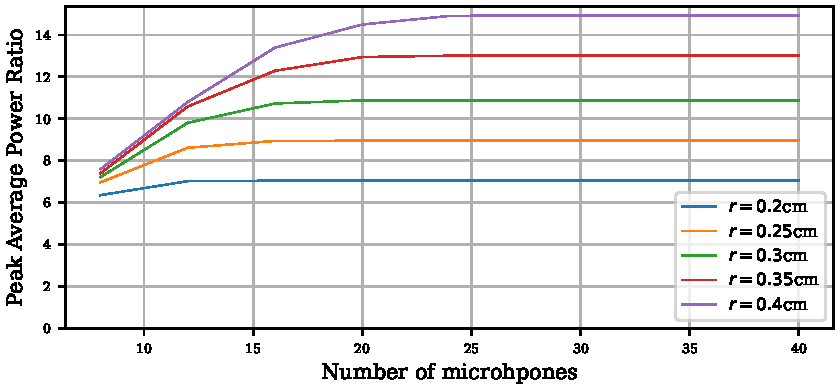
\includegraphics[]{images/5_array_evaluation/circ_m_pap.pdf}
	\caption{PAP ratio for different array radiuses and total number
		of microphones.}
	\label{aev:fig:MicCirc}
\end{figure}
\begin{figure}
	\centering
	%    \includegraphics[width=0.25\textwidth]{mesh}
	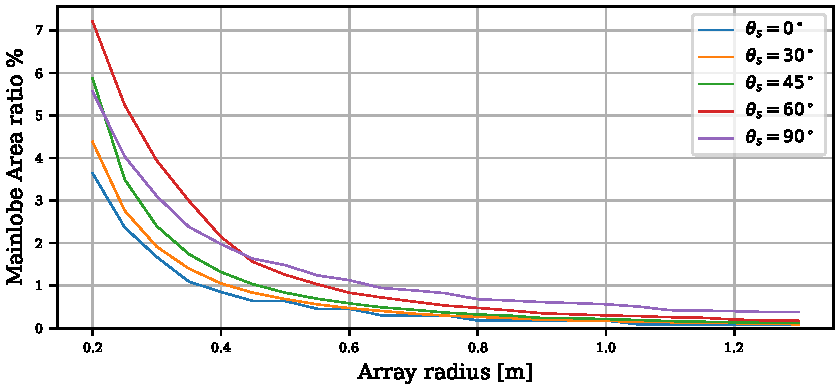
\includegraphics[]{images/5_array_evaluation/area_circ.pdf}
	\caption{Ratio of the mainlobe area compared to the area of a half sphere for
		a circular array with 32 microphones.}
	\label{aev:fig:areaCirc}
\end{figure}
\begin{figure}
	\centering
	%    \includegraphics[width=0.25\textwidth]{mesh}
	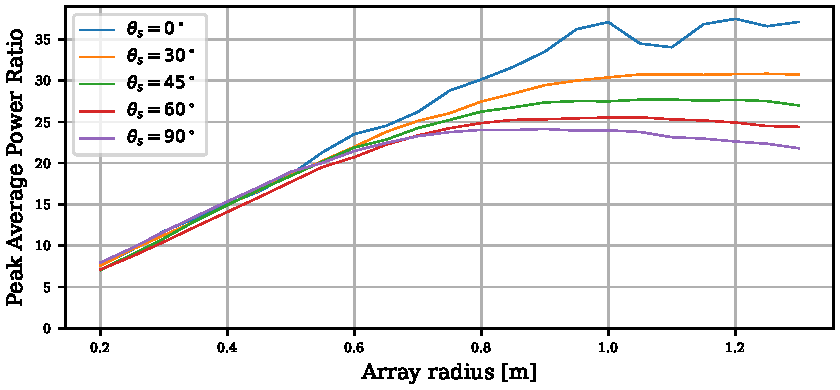
\includegraphics[]{images/5_array_evaluation/PAP_circ.pdf}
	\caption{Peak Average }
	\label{aev:fig:papCirc}
\end{figure}

\subsection{Multi Circular Array}
The multi circualr array is an simplified Undebrink array.
In the original paper, the underbrink array is designed, so that each
microphone covers the same area of a ring with a fixed inner and outer radius and number of circles.
In this thesis the design has been changed so that given the same parameters,
the circle were equally spaced and the phase shift between the circles can be defined.
An example of such an array is shown in Figure \ref*{aev:fig:FancyArr}.

All the parameters together lead to four degrees of freedom when designing such an array.
\begin{figure}
	\centering
	%    \includegraphics[width=0.25\textwidth]{mesh}
	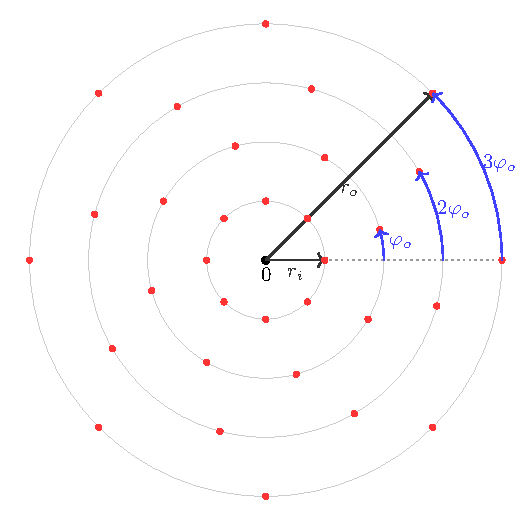
\includegraphics[]{images/5_array_evaluation/fancy_arr.pdf}
	\caption{Hansi.}
	\label{aev:fig:FancyArr}
\end{figure}
Optimizing these four parameter with some mechanical feasibility constraints is not an simple task.
So the effect of single parameters while the others were fixed was studied.
First the amount of circles was set.
Given the 32 microphones, the number of circles is preferred to be a divisor 
of 32.
Four circles seemed like a good balance between number of circles and number of microphones
per circle.

Similar to the circular array, the lower frequencies play a big role in the metrics.
Smaller arrays that have trouble localizing these frequencies perform the worst as seen
in figures \ref*{aev:fig:FancyArea} and \ref*{aev:fig:FancyPap}.

\begin{figure}
	\centering
	%    \includegraphics[width=0.25\textwidth]{mesh}
	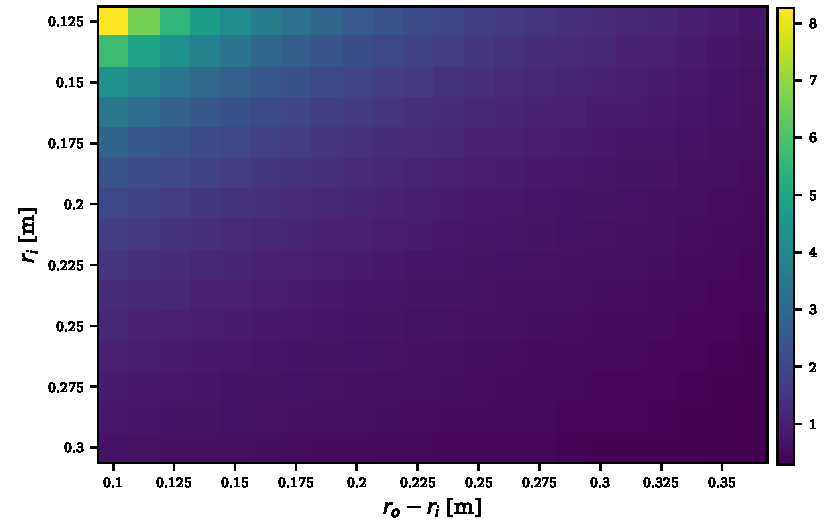
\includegraphics[]{images/5_array_evaluation/fancy_area.pdf}
	\caption{Area of the mainloabe for multi circualr arrays with different
	sizess.}
	\label{aev:fig:FancyArea}
\end{figure}

\begin{figure}
	\centering
	%    \includegraphics[width=0.25\textwidth]{mesh}
	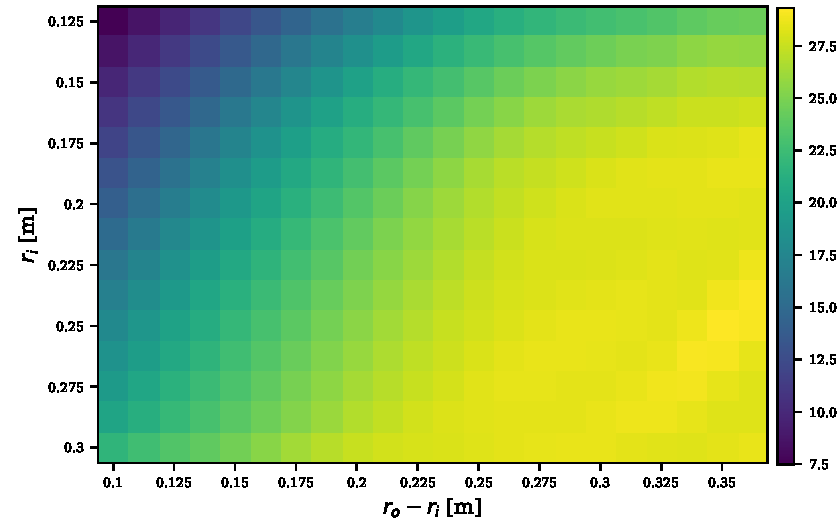
\includegraphics[]{images/5_array_evaluation/fancy_pap.pdf}
	\caption{PAP ratio for multi circualr arrays with different
	sizess.}
	\label{aev:fig:FancyPap}
\end{figure}

To compare this geometry to the circular a maximum radius is set.
In this example 0.4m. 
For a circular array the area ranges from $\approx 0.9\%$ to 
$\approx 2.1\%$ an the PAP ratio is between 14 and 16.
Comparing this to the multicircular array a PAP ratio of up
more than 20 can be reached. 
The areas however are generally larger and can lie in ranges 
betwen one and four percent.

This tradeoff reminds of the windowing functions for discrete
fouriertransforms. 

\subsection{Archimedean Spiral Array}
An archimedean spiral in polar coordinates is defined as
\begin{equation}
	r(\varphi) = a * \varphi.
\end{equation}
Making an array with this shape has three degrees of freedom,
$r$ of the first microphone, $r$ of the last microphone and the 
spiral arm spacing $a$. 



\newpage
\section{Mechanical Design}
The mechanical design of the array prototypes was centered around the objective of testing a wide range of array configurations.
To achieve this, two flexible microphone array frames were developed.
A significant aspect of the design process involved determining the overall size of the arrays.
While larger arrays typically offer better performance, practicality and manufacturability had to be considered as well.
In practice, a maximal outer diameter of 60\,cm was chosen for the array prototypes.
Based on simulation results, two specific array types were explored: The Multi-Circular Array and the Archimedean Spiral Array, as described in the next sections.

\subsection{Multi-Circular Array}
\begin{minipage}{\linewidth}
	\begin{wrapfigure}{r}{7.5cm}
		\vspace{-0.8cm}
		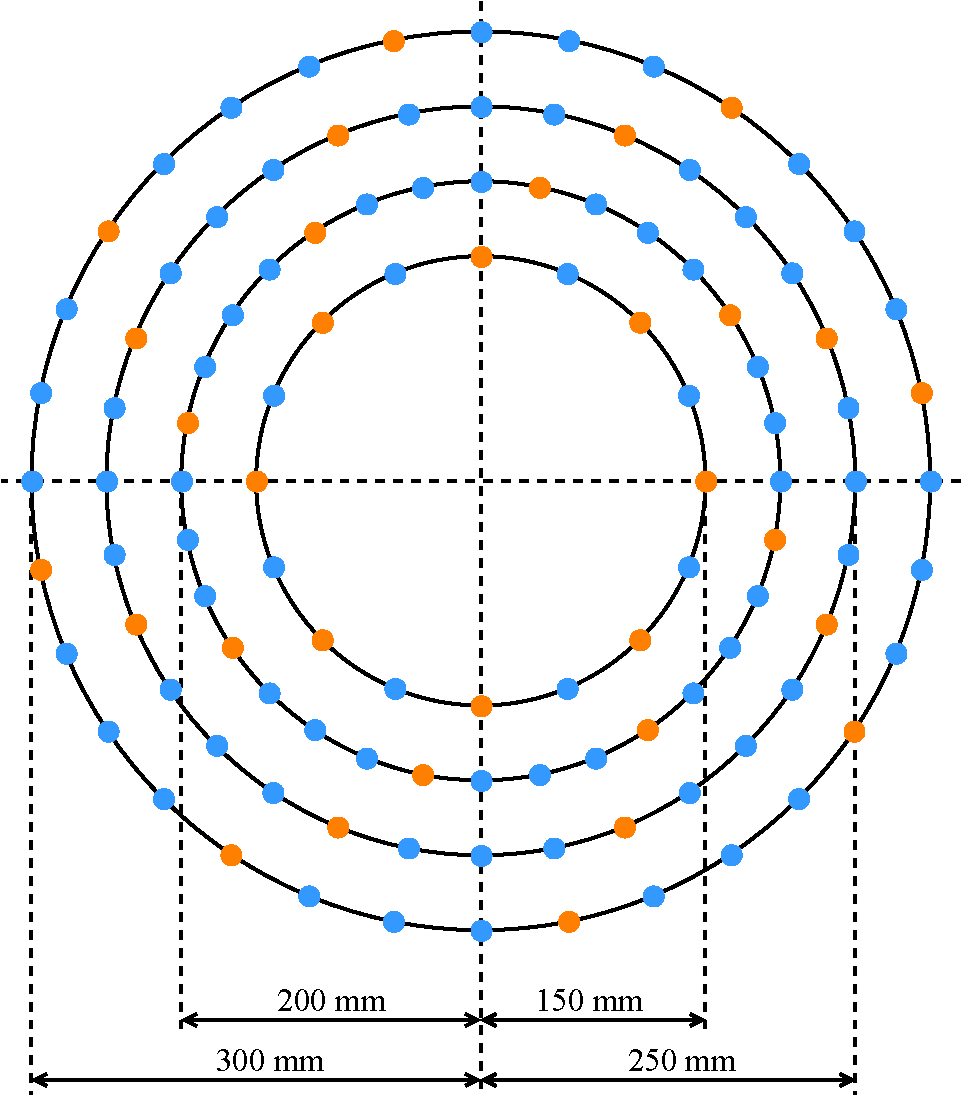
\includegraphics[width=7cm]{images/5_array_evaluation/prototype_array_multi_circular.pdf}
		\centering
		\caption{Multi-Circular Array}
		\label{fig:prototype_array_multi_circular}
	\end{wrapfigure}
	This array geometry allows to build circular arrays with radiuses of 20cm, 25cm and
	30cm.
	A circle with a radius of 15cm was added to make the adaptation of the Underbrink array. 
	The orange points show such a configuration with $\phi_o = \pi/16$.
	A second geometry, where each circle is shifted by $\phi_o = \pi / 8$ is also possible.
\end{minipage}
\vspace{5.5cm}    % Adjust this depending on the length of the text above

\subsection{Archimedean Spiral Array}
\begin{minipage}{\linewidth}
	\begin{wrapfigure}{r}{7.5cm}
		\vspace{-0.8cm}
		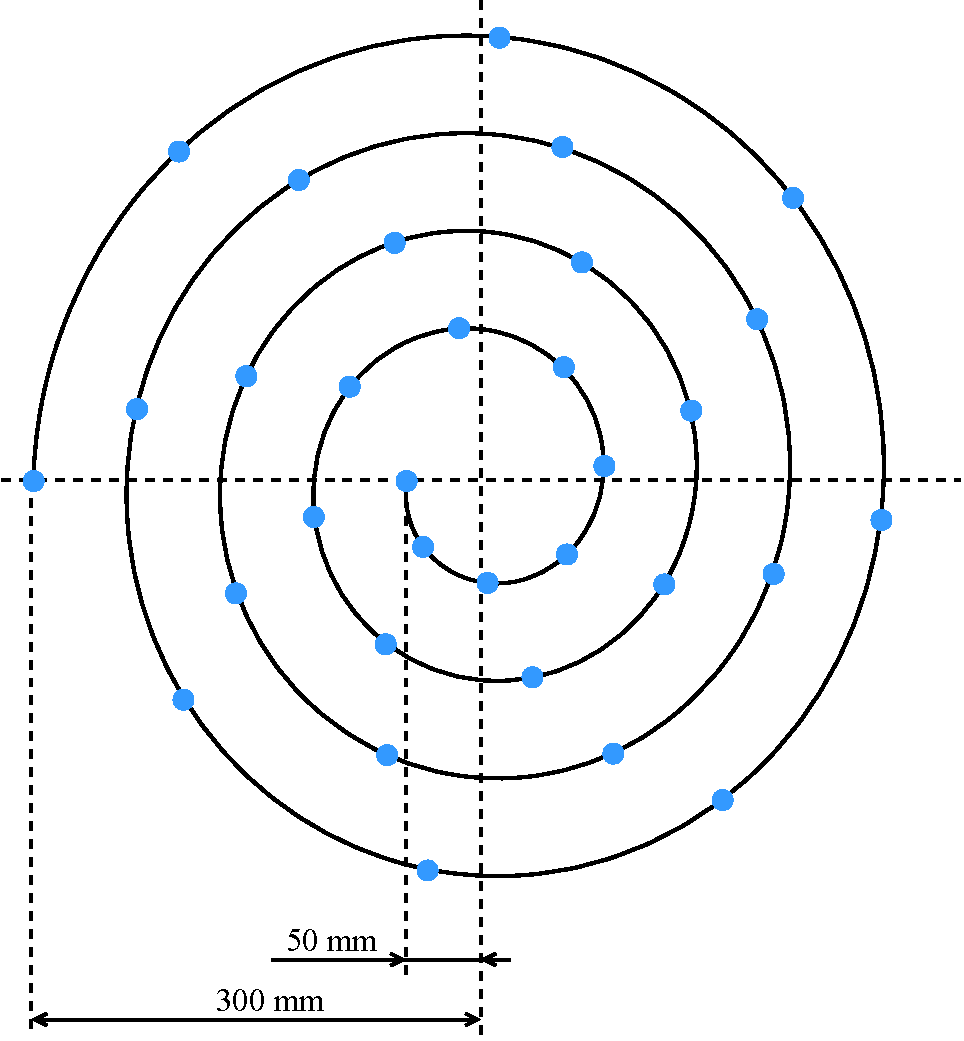
\includegraphics[width=7cm]{images/5_array_evaluation/prototype_array_archimedian_spiral.pdf}
		\centering
		\caption{Archimedean Spiral Array}
		\label{fig:prototype_array_archimedian_spiral}
	\end{wrapfigure}
	The archimedean Spiral Array was made with a inner radius of 5cm and an outer radius of 
	30cm. The spiral makes a total of four turns which leads to a 
	separation distance of 6.25cm.

\end{minipage}
\newpage


\subsection{Wooden Prototype Arrays}
Two wooden prototypes, a multi-circular array and an Archimedean spiral array, were manufactured by laser-cutting 5\,mm plywood.
Both arrays had to be split into several pieces due to the limited size of the laser-cutter and were later glued together.
In the centre of each array, a mechanical mount for the Acquisition-System hardware was integrated.
\begin{figure}[h!]
	\centering
	\begin{minipage}{0.49\textwidth}
		\centering
		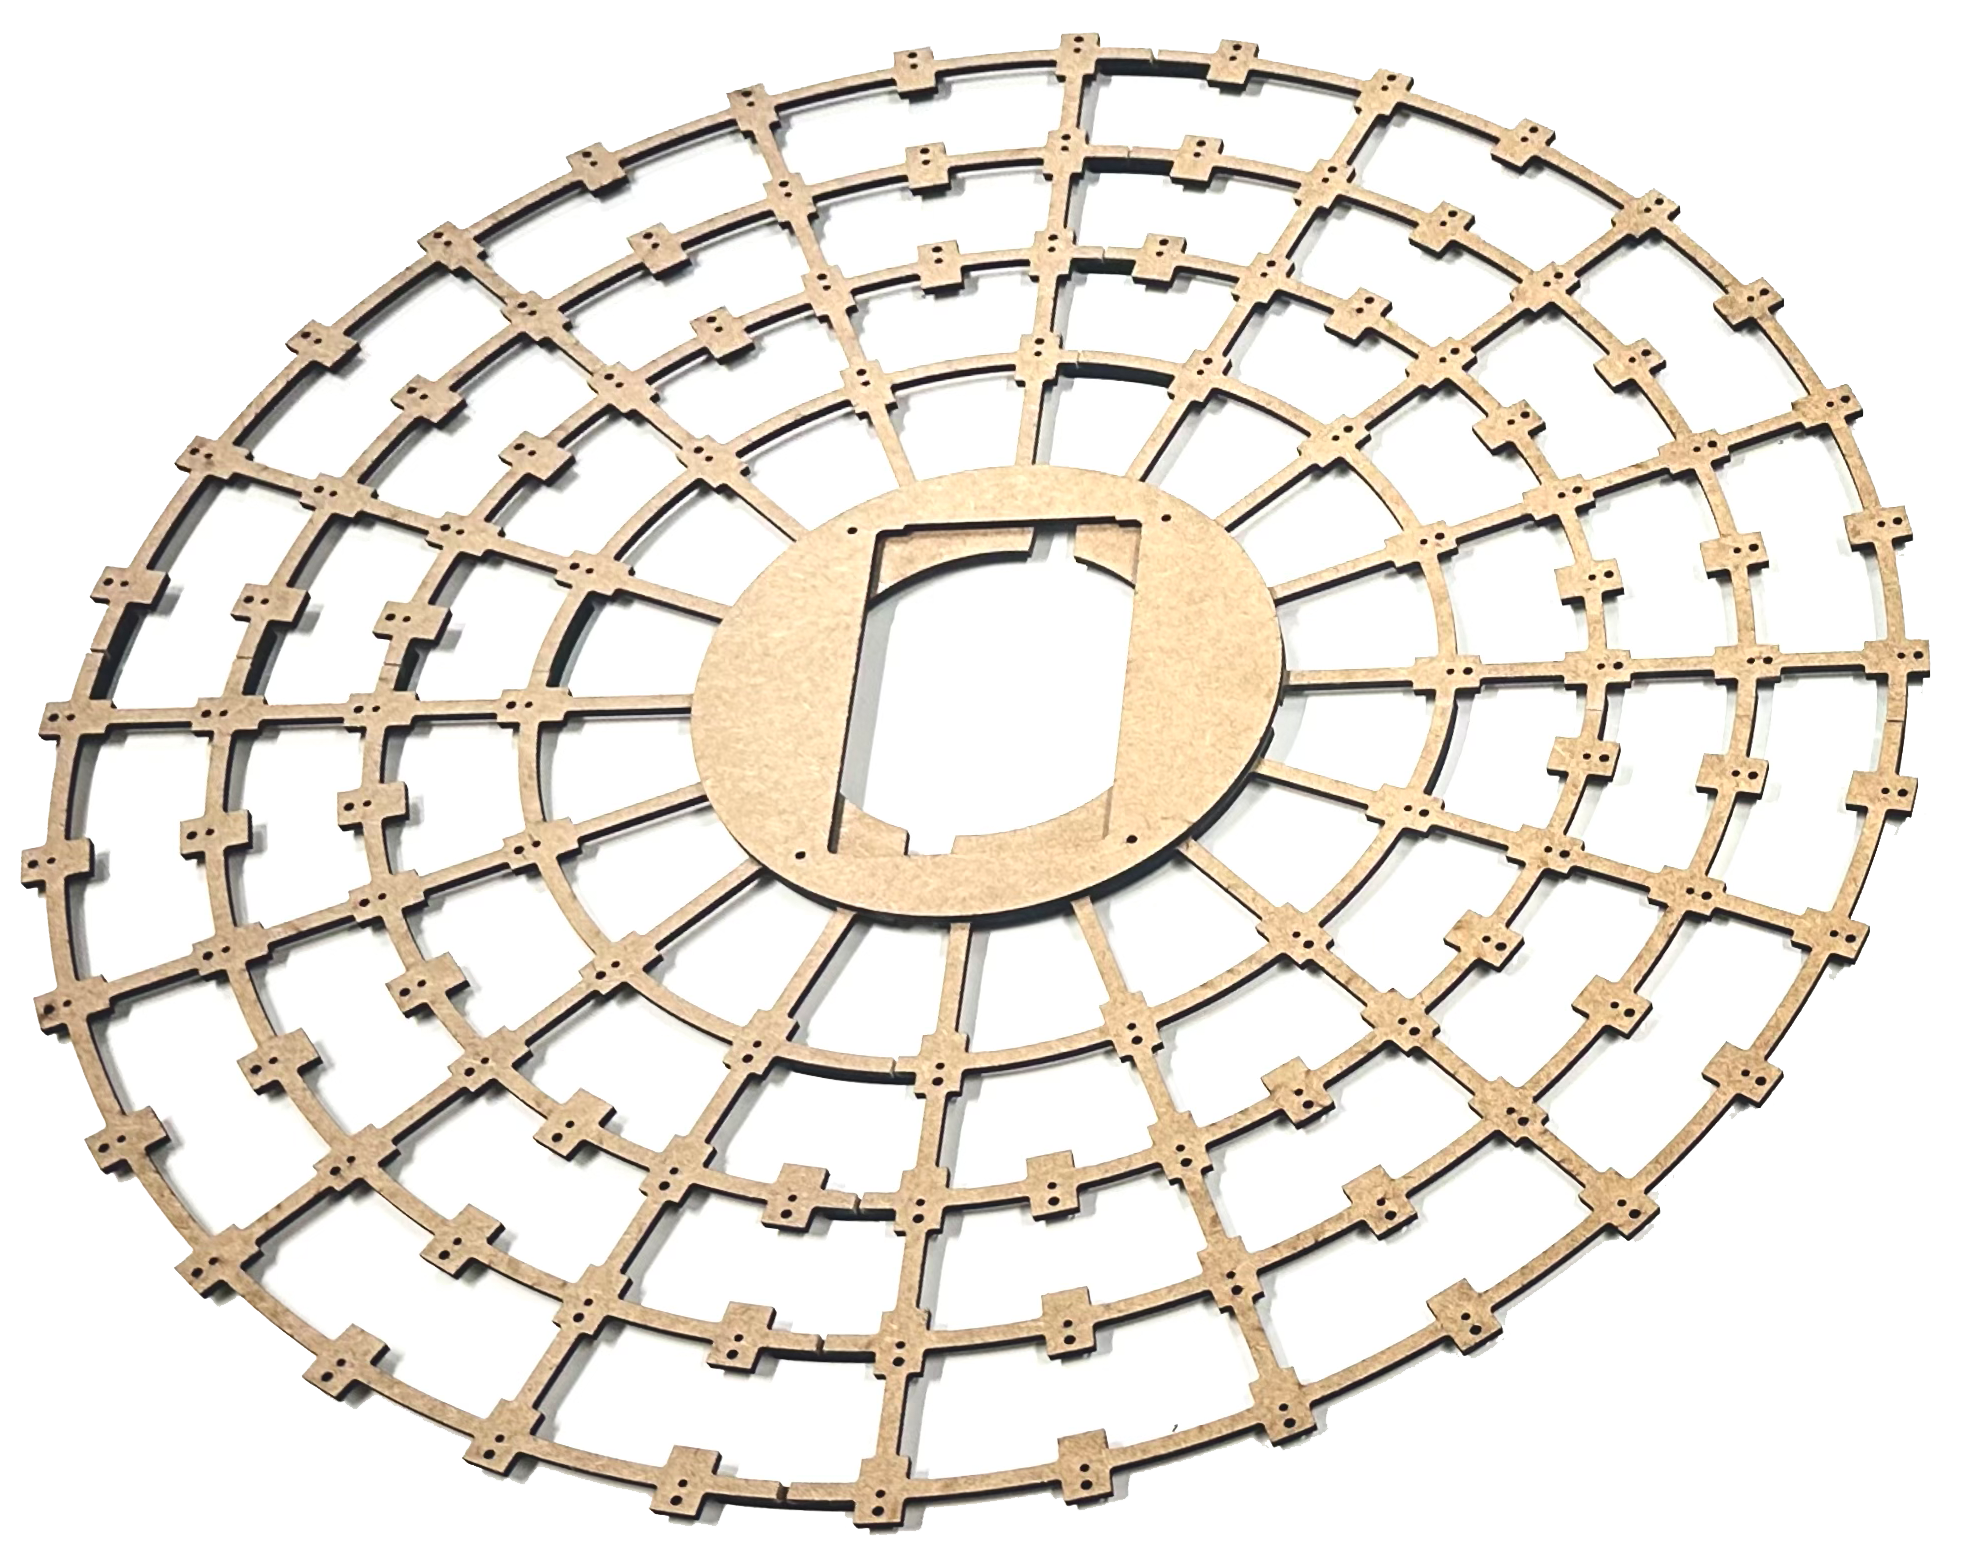
\includegraphics[width=0.95\textwidth]{images/5_array_evaluation/wooden_circular_array.png}
		\caption{Wooden Circular Array}
		\label{fig:wooden_circular_array}
	\end{minipage}
	\begin{minipage}{0.49\textwidth}
		\centering
		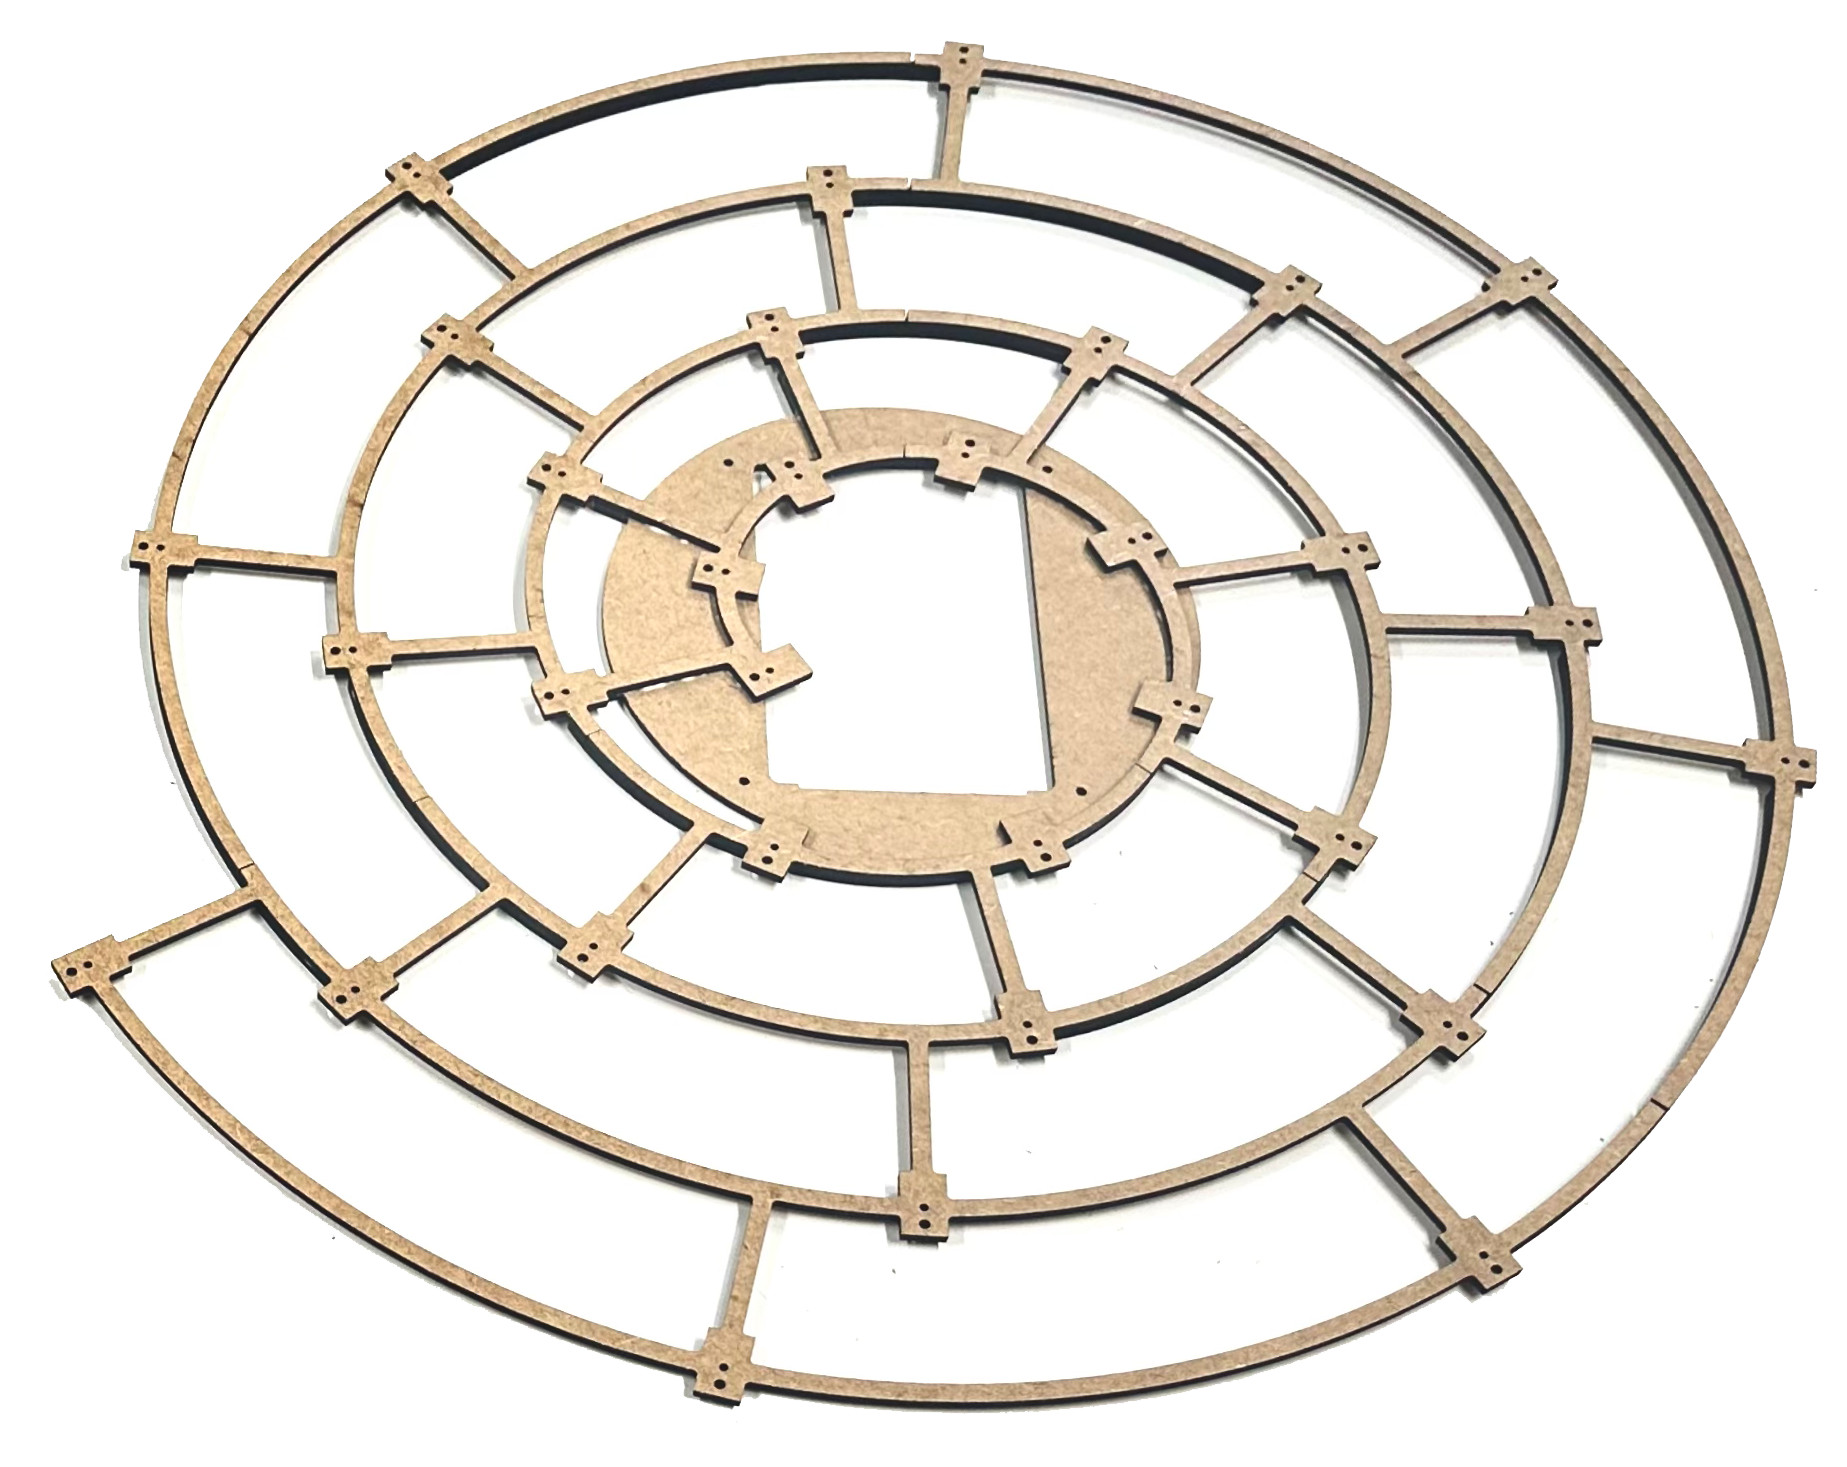
\includegraphics[width=0.95\textwidth]{images/5_array_evaluation/wooden_archimedean_spiral_array.png}
		\caption{Wooden Archimedean Spiral Array}
		\label{fig:wooden_archimedean_spiral_array}
	\end{minipage}
\end{figure}

\section{Measurements \& Findings} \label{sec:array_prototype_measurements}
The performance of the physical arrays were evaluated with outdoor measurement.
To simulate a drone the sound of a DJI Mavic drone \todo{Cite yt} was played back on 
UE BOOM loudspeakers.
Various angles were tested by turning and tilting the array such that 
the loudspeakers are in the direction to bes tested.
The distance of the loudspeaker to the array was set to 
15m.
All of the tests except the archimedean were made in an open field with little reverberation.
The archimedean array had to be tested between buildings due to rain.

During the first tests, the wind caused the microphone to overdrive
thus making the signal useless.
To reduce this a RØDE DeadWombat microphone cover was cut into small pieces
and glued onto the microphones.
This lead to significantly less wind noises.
Two examples of test configurations are depicted in Figure \ref*{fig:testSetup}.
The measured data was then evaluated using the mainlobe area and PAP ratio. 
Additionaly to compare the real arrays to the simulated one, each measurement
was also simulated.
The result for a $\theta = 90^\circ$ and $\theta = 30^\circ$ are shown in 
Figure \ref*{fig:TestSim}.
In most cases the simulated arrays performed better.
This is probably due to lower background noise in the environment and other 
Quite extreme differences can be seen with the Archimedean array which is 
suspected to be caused by the more reverberant measurement environment.

\begin{figure}[]
	\centering
	\begin{subfigure}[b]{0.49\textwidth}
		\centering
		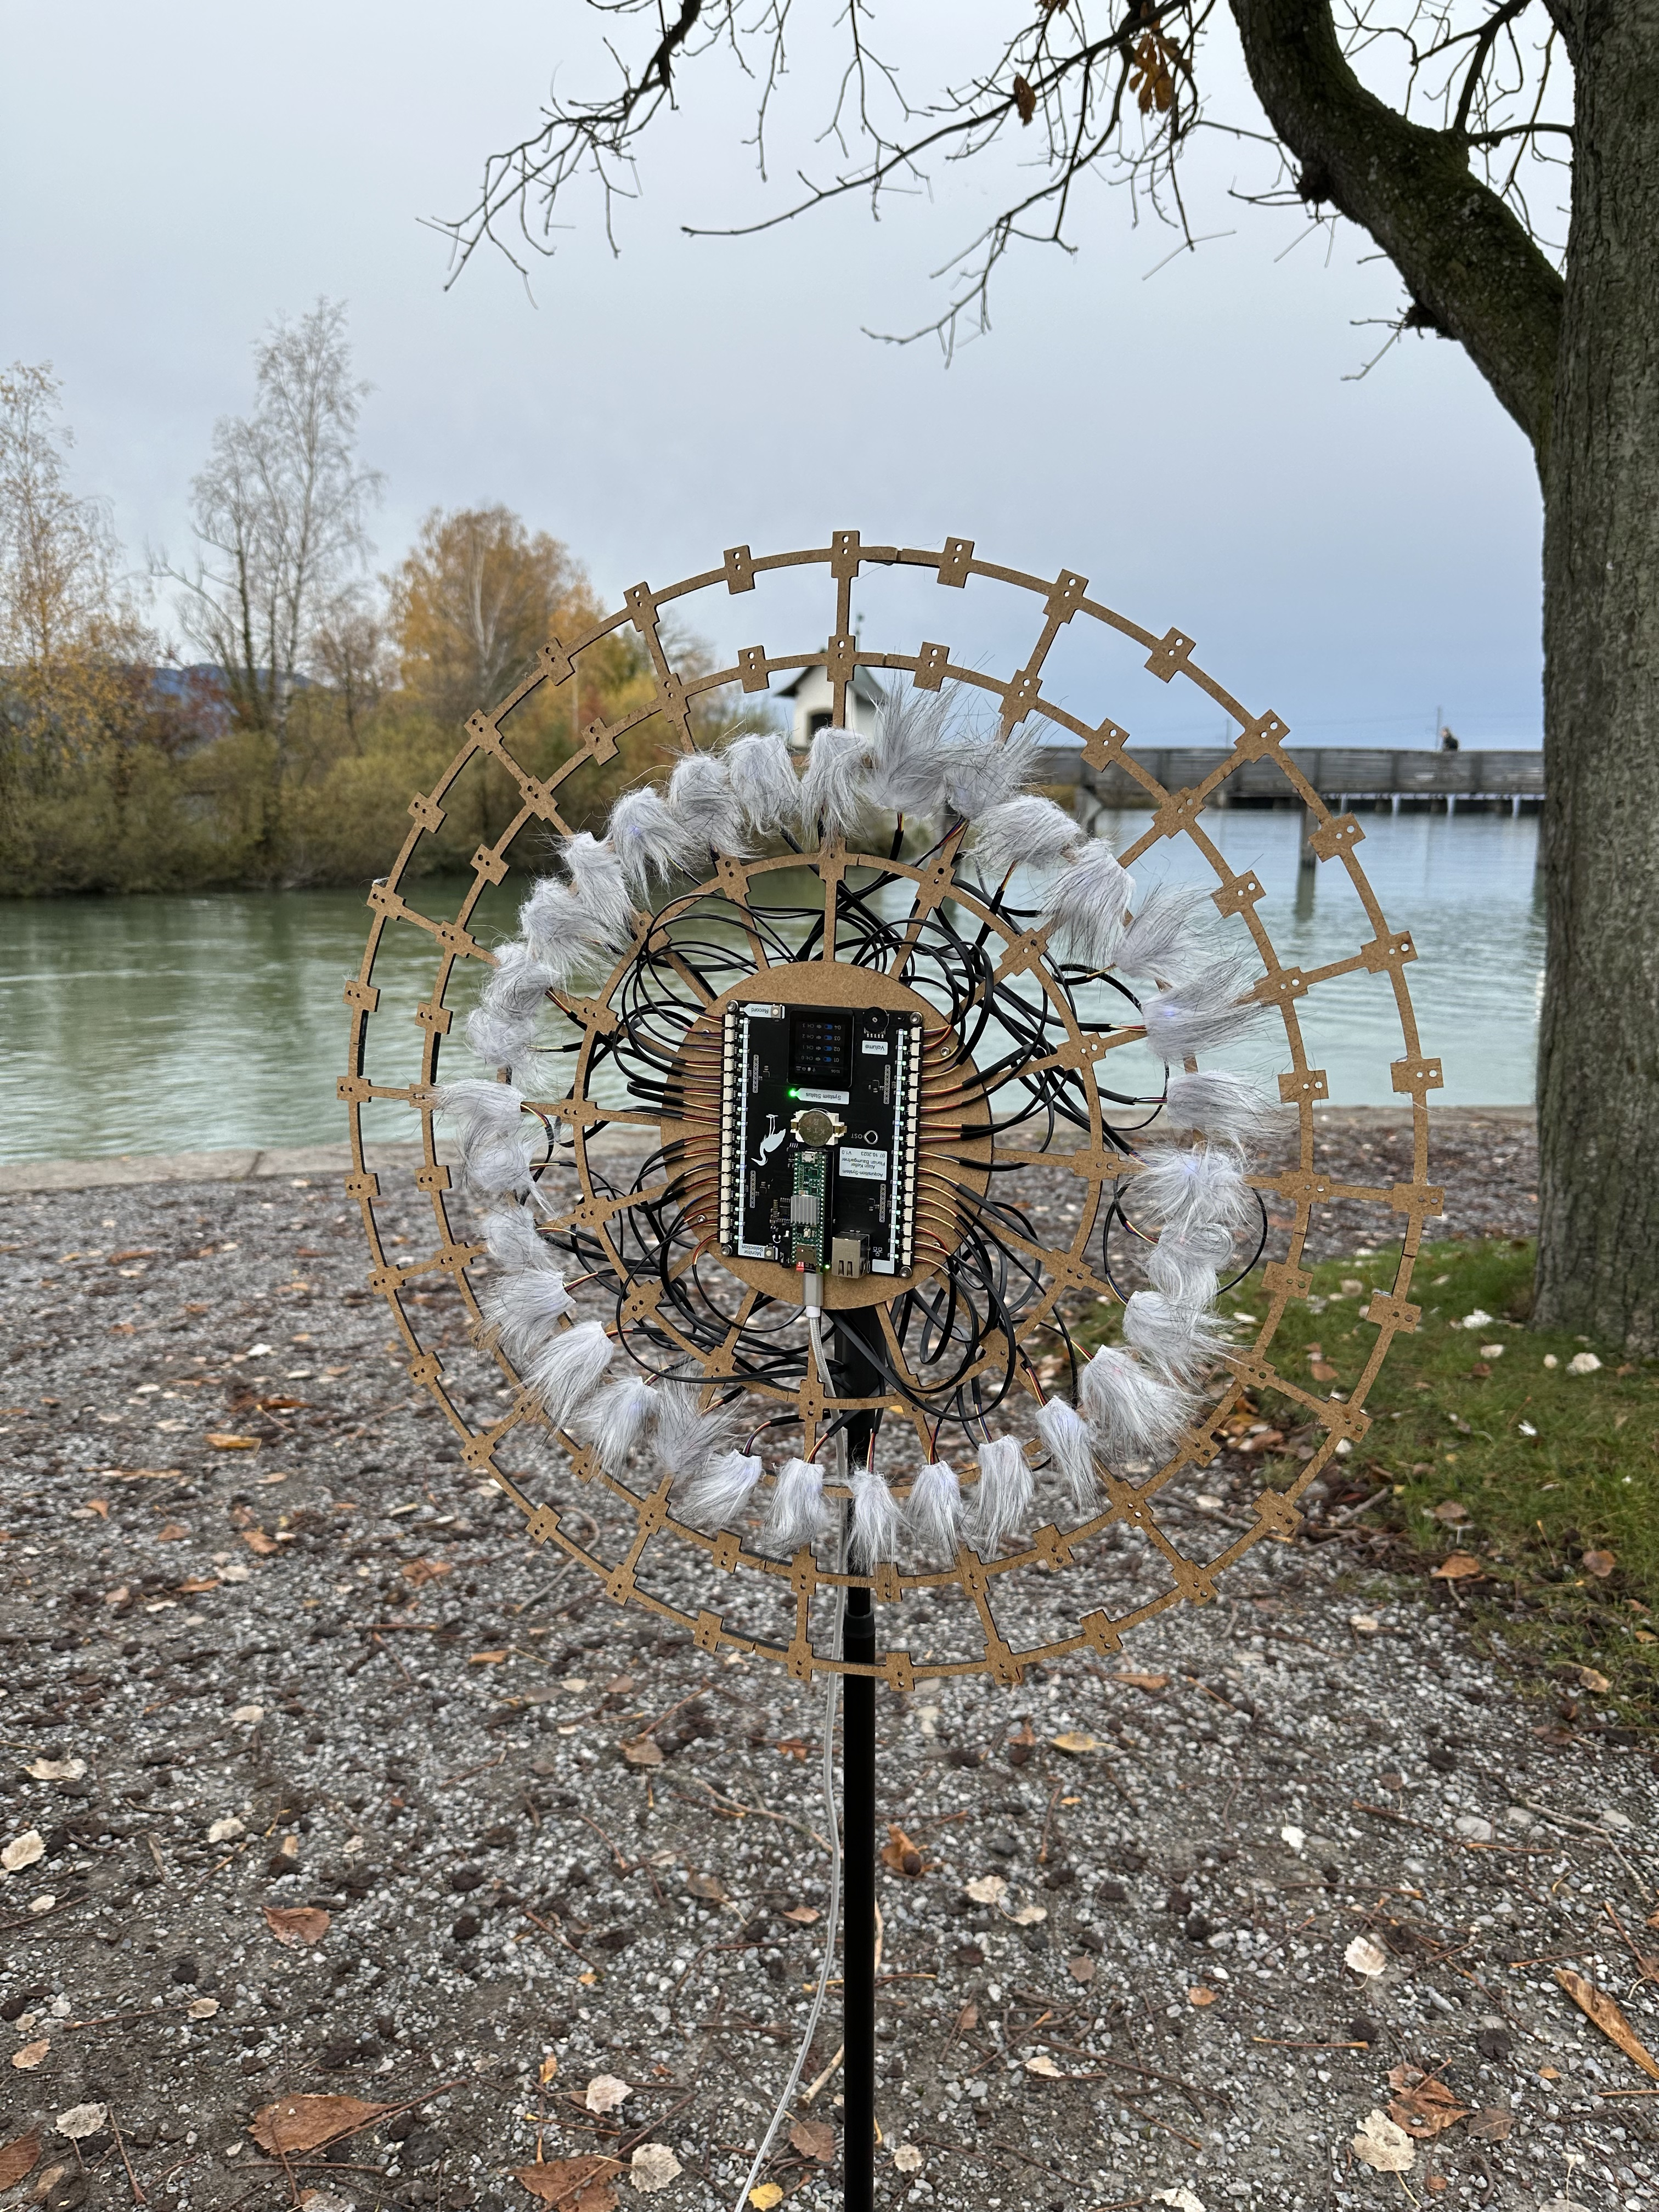
\includegraphics[width=0.95\textwidth]{images/5_array_evaluation/array_test_1.jpg}
		\caption{Multi-Circular Array (inner circle)}
		\label{fig:array_test_1}
	\end{subfigure}
	\begin{subfigure}[b]{0.49\textwidth}
		\centering
		\includegraphics[width=0.95\textwidth]{images/5_array_evaluation/array_test_2.jpg}
		\caption{Multi-Circular Array (interleaved  pattern)}
		\label{fig:array_test_2}
	\end{subfigure}
	\caption{Test arrays.}
	\label{fig:testSetup}
\end{figure}

\begin{figure}[]
	\centering
	\begin{subfigure}[b]{1\textwidth}
		\centering
		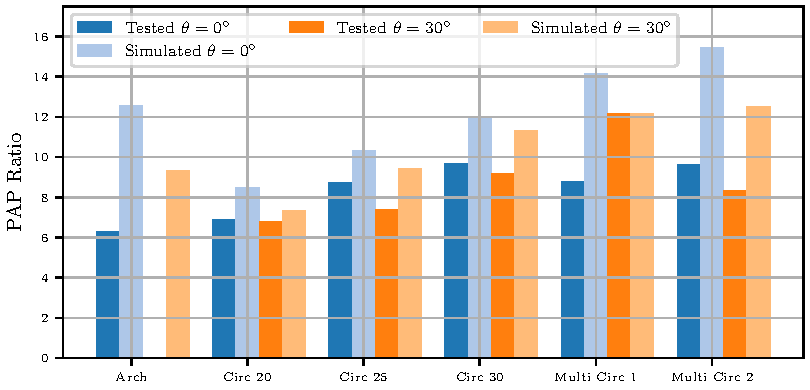
\includegraphics[width=0.95\textwidth]{images/5_array_evaluation/PapTestSim.pdf}
		\caption{Comparison of the PAP ration.}
		\label{fig:comp1}
	\end{subfigure}
	\begin{subfigure}[b]{1\textwidth}
		\centering
		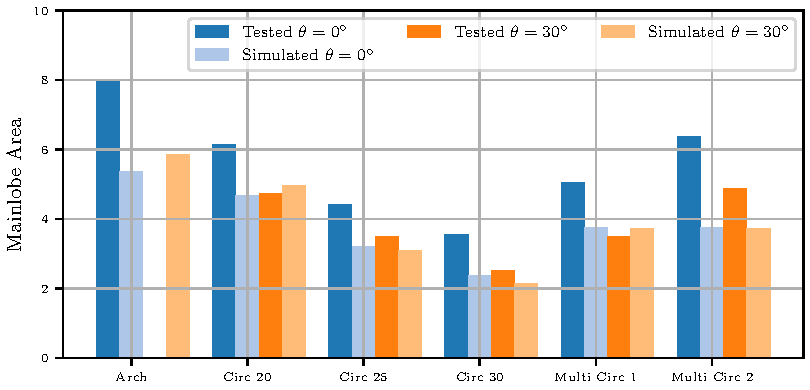
\includegraphics[width=0.95\textwidth]{images/5_array_evaluation/AreaTestSim.pdf}
		\caption{Comparison of the mainlobe area}
		\label{fig:comp2}
	\end{subfigure}
	\caption{Measurements and simulation comparisons with a a source located at $(r, \phi, \theta) = (15, 0, \pi/2)$}
	\label{fig:TestSim}
\end{figure}

All the two dimensianal array geometries tested have the drawback
that their performance is dependent on the \acrshort*{doa}.
A directional independent array design is the spherical array. \cite{keylist}
It uses the theory of spherical harmonics to sample the sound at specific points
on a sphere.
The number of microphones used is depending on the order of the harmonics and so 
is the beam pattern.
It was decided to not build such a spherical array due to its mechanical 
challenging geometry.

Expanding the idea of a three dimensional geometry several other
possible advantages come to light.
Until now the measurement space is a semisphere above the array with the array as the cutting surface.
This can lead to ambiguity, when a sound source is under the array.
The beamforming delays are the same for a source mirrored at the cutting surface.
A three dimnsional array does not have this problem.



\newpage
\section{Final Array Geometry} \label{sec:final_array_geometry}
Finally the idea of a multicircular array where the circles can be 
set to a different height came up.
In the measurements the multicircual array performed well. 
To get an optimal array geometry, the maximal radius of 0.38m was first set.
Even though a larger radius would yield better results, it also
comes with more mechanical challanges.
The angle $\phi_o$ chosen to be the same as in the test array
\textit{Multicircualr array 1} as it perfromed the best of the two multicircular 
configurations.
To find a suited $r_i$, the mainlobe area and PAP ratio was calculated for
various $r_i$.
The results are depicted in Figure \ref*{fig:finflat}.
Figure \ref{fig:finpap} shows that the PAP does not 
steadily increase but rather peak at a specific radius and then
begins to decrease again.
A $r_i$ of 0.2m was chosen since it is a good tradeoff between 
mainlobe area and PAP ratio.
Figure \ref*{fig:final_array_concept_design} shows the final
properties of the array.

\begin{figure}[h!]
	\centering
	\begin{subfigure}[b]{1\textwidth}
		\centering
		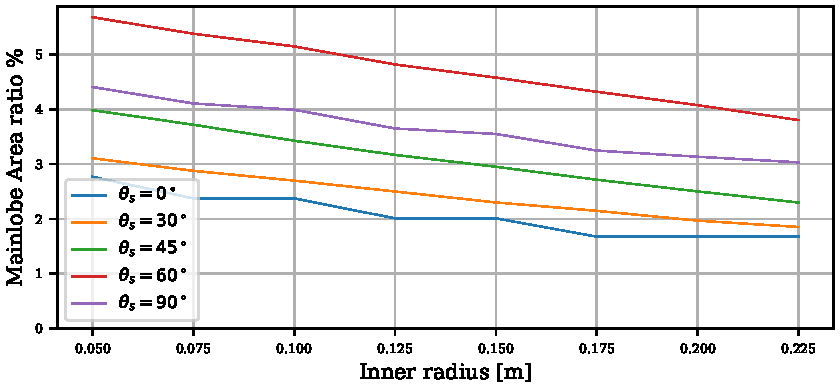
\includegraphics[width=0.95\textwidth]{images/5_array_evaluation/final_flat_area.pdf}
		\caption{GG}
		\label{fig:finar}
	\end{subfigure}
	\begin{subfigure}[b]{1\textwidth}
		\centering
		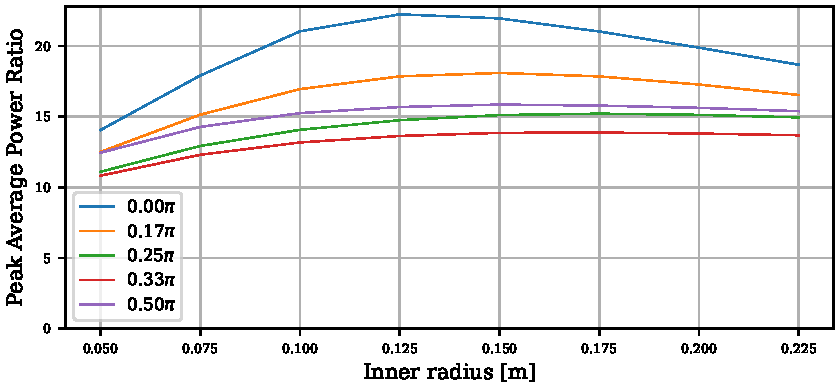
\includegraphics[width=0.95\textwidth]{images/5_array_evaluation/final_flat_PAP.pdf}
		\caption{EZ}
		\label{fig:finpap}
	\end{subfigure}
	\caption{Test and simulation comparisons with a a source located at $(r, \phi, \theta) = (15m, 0^\circ, 90^\circ)$}
	\label{fig:finflat}
\end{figure}

\begin{figure}[h]
	\centering
	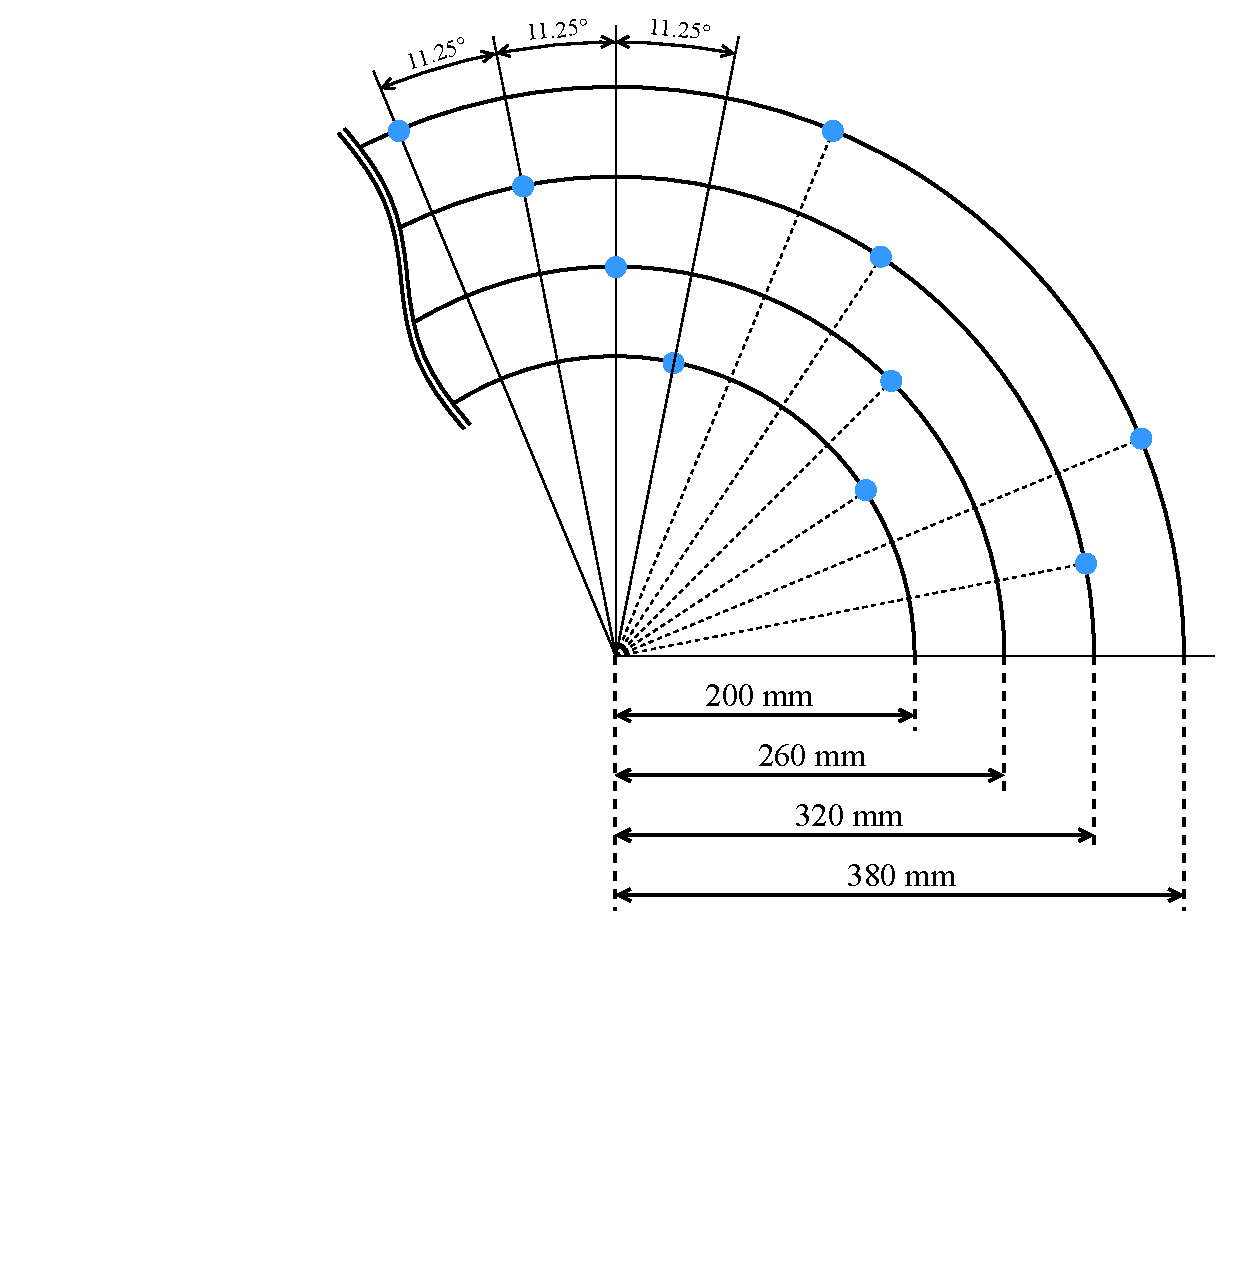
\includegraphics[width=0.75\textwidth, trim={5.5cm 6.0cm 0 0}]{images/5_array_evaluation/final_array_concept_design.pdf}
	\caption{Final Array Concept Design}
	\label{fig:final_array_concept_design}
\end{figure}


To make the circular sub array on different height levels
a mechanical system is used as discribed in Section \ref{chap:fin:Mech}.
The performance of the array changes with the angle of the microphone arms.
Since a bigger angle lowers the distances between the microphones it is to be 
excpected, that the performance decreases due to the influence of the lower frequencies.
Figure \ref*{fig:fintilt} shows how the metrics change with the arm angle.
Up to an angle of $30^\circ$ performance decreases slowly.
Therefore the optimal angle range is between 0 and 30 degrees.

\begin{figure}[h!]
	\centering
	\begin{subfigure}[b]{1\textwidth}
		\centering
		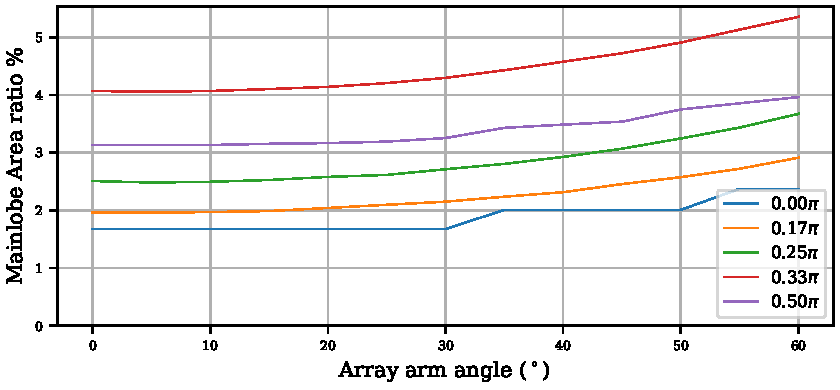
\includegraphics[width=0.95\textwidth]{images/5_array_evaluation/tilt_area.pdf}
		\caption{GG}
		\label{fig:finartilt}
	\end{subfigure}
	\begin{subfigure}[b]{1\textwidth}
		\centering
		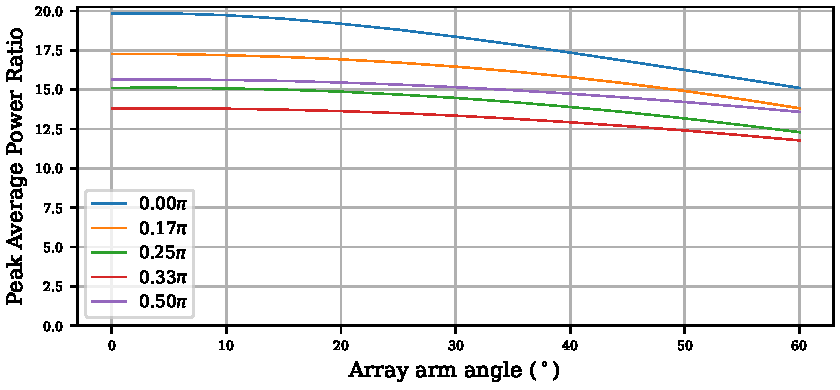
\includegraphics[width=0.95\textwidth]{images/5_array_evaluation/tilt_PAP.pdf}
		\caption{EZ}
		\label{fig:finpaptilt}
	\end{subfigure}
	\caption{Test and simulation comparisons with a a source located at $(r, \phi, \theta) = (15, 0, \pi/2)$}
	\label{fig:fintilt}
\end{figure}


